\documentclass{article}
\usepackage[pdftex]{graphicx}
\usepackage{amsmath}
\usepackage{verbatim}
\usepackage{enumerate}
\author{Michael Anderson}
\title{Takehome Final}
\begin{document}
\maketitle
\center{CS533}
\center{Prof. Fern}\\
\flushleft
\newpage

\section{}
Imagine a k-order MDP in which all states have at most one parent state. In
other words, for all $s'$ that are states in the MDP, there exists at most one
$s$ such that $T(s,a,s') > 0$. Such a a k-order MDP would be directly
convertible to a first-order MDP, because each state would only have one
possible vector of ancestor states.

\vspace{1em}

However, in an average k-order MDP where states can have multiple parents,
a state could have a number of different ancestor vectors, and that information
is not really accounted for in a normal first-order MDP.

\vspace{1em}

So, to convert a k-order MDP $M$ to a first-order MDP $M'$, traverse M cloning
states, actions, rewards, and transitions over to $M'$ exactly, except
whenever a state $s$ is found with multiple parents, make a set of states in
$M'$, ${s_1,s_2,...}$, one state for each of the parents to transition to. Also
duplicate all of the descendants of $s$, so that $s_1,s_2,...$ each have their
own copy. Finally, when copies of descendants are made in this way, check to
see if they can be merged back together farther down the tree when they have the
same ancestor vectors again (see picture).

\vspace{1em}

The handling of $A'$, $R'$, and $T'$ are straightforward. For states without
multiple
parents, they are identical to $A$, $R$, and $T$. But supposing that for some
state
$s'$ in S there exists multiple $s$ such that $s$ is in $S$ and $T(s,a,s') > 0$,
then for each such $s$ with a corresponding $a$ that reaches $s'$, make $a$ a
member of $A'$ and make $T'(s,a,s_i) = T(s,a,s')$. For the rewards, make
$R'(s_i) = R(s')$.

\vspace{1em}

Below is an example of part of a 3-order MDP $M$ and the corresponding part of
its equivalent first-order MDP $M'$. This MDP is deterministic for simplicity,
but without loss of generality.
States are labeled 1 through 9 in $M$, and
in $M'$ states are labeled by their grandfather, their father, and then the
state themselves. Notice that since 5 and 6 have two parents, they are each
expanded into two states in $M'$. 7 is expanded into four states, because it
has four combinations of grandfather/father pairs. 8 only has two such
combinations and 9 only has one, so we see in the picture an example of the
merging of descendant states mentioned above. 

\newpage

\begin{center}

$M$
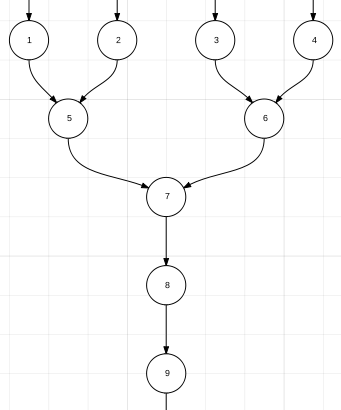
\includegraphics[scale=0.85]{M.png}

\vspace{5em}

$M'$
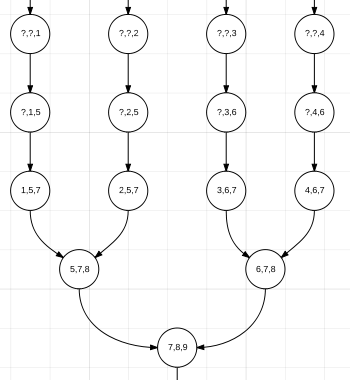
\includegraphics[scale=0.85]{M_prime.png}

\end{center}

\section{}

\newpage

\section{}

Assume the worst case, which is that the maximum reward $R_{max}$ is obtained
at each level of the tree. Then at search depth h, the reward is
$\beta^h R_{max}$, because $R_{max}$ is discounted by a factor of $\beta$ at
each level. The infinite horizon reward becomes an easily simplifiable
geometric series:

\[
Q_\pi(s,a) = \sum_{i = 1}^{\infty} \beta^i R_{max} =
\frac{1}{1-\beta}R_{max}
\]

The finite horizon reward then, for a horizon of $h$, is

\[
Q_\pi(s,a,h) = \sum_{i = 1}^{h} \beta^i R_{max} = 
\frac{1-\beta^h}{1-\beta}R_{max}
\]

Since this is the worst case, the difference between $Q_\pi(s,a)$ and
$Q_\pi(s,a,h)$ is maximized by:

\[
\frac{1}{1-\beta}R_{max} - \frac{1-\beta^h}{1-\beta}R_{max} =
\frac{\beta^h}{1-\beta}R_{max}
\]

\newpage

\section{}
\begin{enumerate}[(a)]
\item


\item

\end{enumerate}

\newpage

\section{}

\end{document}
